\documentclass[notheorems,envcountsect,allowframebreaks,xcolor=svgnames,8pt]{beamer}

\def\PM{{\mathrm{PM_{2.5}}}} 
\definecolor{uniblue}{rgb}{.125,.25,.5}
\def\cub{\color{uniblue}}

\usepackage[english]{babel}
\usepackage[utf8]{inputenc}
\usepackage{times}
\usepackage[T1]{fontenc}
\usepackage{bookmark}
\usepackage{amsmath}
\usepackage{bbold}
\usepackage{graphicx}
\usepackage{subfigure}
\usepackage{multimedia}
\usepackage{hyperref}
\usepackage{xcolor}

%%%special symbols%%%

\newcommand{\IS}{\mathbb{S}}
\newcommand{\U}{{\bf U}}
\newcommand{\V}{{\bf V}}
\newcommand{\W}{{\bf W}}
\newcommand{\NN}{\mathbb{N}}
\newcommand{\RR}{\mathbb{R}}
\newcommand{\QQ}{\mathbb{Q}}
\newcommand{\ZZ}{\mathbb{Z}}
\newcommand{\CC}{\mathbb{C}}
\newcommand{\FF}{\mathbb{F}}
\newcommand{\SSS}{\mathfrak{S}}
\newcommand{\dd}{\mathfrak{d}}
\newcommand{\LL}{\mathcal{L}}
\newcommand{\Lie}{\text{Lie}}
\newcommand{\GG}{\mathcal{G}}
\newcommand{\AAA}{\mathcal{A}}
\newcommand{\PPP}{\mathcal{P}}
\newcommand{\res}{\text{res}}
\newcommand{\Mat}{\text{Mat}}
\newcommand{\mm}{\mathfrak{m}}
\newcommand{\RRR}{\mathcal{R}}
\newcommand{\OOO}{\mathcal{O}}
\newcommand{\Conj}{\mbox{Conj}}
\newcommand{\Syl}{\mbox{Syl}}
\newcommand{\Mod}{\mbox{ mod }}
\newcommand{\Aut}{\mbox{Aut}}
\newcommand{\Char}{\mbox{ char }}
\newcommand{\ZZZ}{\mathcal{Z}}
\newcommand{\oo}{$\ddot{\mbox{o}}$}
\newcommand{\Tor}{\mbox{Tor}}
\newcommand{\Hom}{\mbox{Hom}}
\newcommand{\stt}{^{\mbox{\tiny{st}}}}
\newcommand{\ndd}{^{\mbox{\tiny{nd}}}}
\newcommand{\rdd}{^{\mbox{\tiny{rd}}}}
\newcommand{\thh}{^{\mbox{\tiny{th}}}}
\newcommand{\Gal}{\mbox{Gal}}
\newcommand{\ii}{\mathfrak{i}}
\newcommand{\bbox}{\hfill $\blacksquare$}
\newcommand{\ep}{\\ \vspace{.001cm}}
\newcommand{\xx}{\mathbf{x}}
\newcommand{\cnn}{\mathbb{C}^{n \times n}}
\newcommand{\diag}{\mbox{Diag}}
\newcommand{\agl}{AGL(2,\ZZ)}
\newcommand{\gl}{GL(2,\ZZ)}
\newcommand{\ord}{\operatorname{ord}}
\newcommand{\lcm}{\operatorname{lcm}}


\definecolor{cornellred}{rgb}{0.75, 0.01, 0.1}

\mode<presentation> {
  \useoutertheme[footline=authorinstitutetitle]{miniframes}
  \usetheme{Darmstadt}
  \usecolortheme[named=cornellred]{structure}
  \setbeamercovered{transparent}
  \setbeamertemplate{navigation symbols}{}
  \setbeamertemplate{theorem}[ams style]
  \setbeamertemplate{theorems}[numbered]
  \setbeamercolor{frametitle}{fg=structure}
  \setbeamertemplate{frametitle}{
    \raggedleft
    {\bf \insertframetitle}
    \par
  }
}

\newtheorem{theorem}{Theorem}
\newtheorem{definition}{Definition}
\newtheorem{proposition}{Proposition}
\newtheorem{corollary}{Corollary}
\newtheorem{lemma}{Lemma}
\newtheorem{example}{Example}
\newtheorem{examples}{Examples}
\newtheorem{remark}{Remark}
\newtheorem{question}{Question}

\title[Fusing AOD and PM$2.5$ datasets]
{Fusing surface and satellite-derived PM observations to \\ determine the impact of international transport on coastal PM$_{2.5}$ concentrations in the western U.S.}

\author
{Neha Bora \and Tuo Chen \and Dana Cochran \and Kelly Dougan \and Guatam Sabnis \and Chuanping Yu}

\institute[SAMSI]
{Industrial Math/Stat Modeling Workshop \\ Environmental Protection Agency}

\subject{Talks}

%\AtBeginSubsection[] {
%  \begin{frame}<beamer>{Outline}
%  \tableofcontents[currentsection,currentsubsection]
%  \end{frame}
%}
\AtBeginSection[]
{
 \begin{frame}<beamer>
 \frametitle{Outline}
 \tableofcontents[currentsection]
 \end{frame}
}

\begin{document}

\begin{frame}
\titlepage
\end{frame}

%\begin{frame}{Outline}
%\tableofcontents
%% You might wish to add the option [pausesections]
%\end{frame}
%------------------------------------------Introduction--------------------------------------------------------
\section{Introduction}
\iffalse
\begin{frame}{What we plan to talk about}
\begin{itemize}
\item Background

\begin{itemize}
\item What are PM$_{2.5}$ and AOD?
\end{itemize}

\item The Problem
\begin{itemize}
\item Can we use PM measurements to predict past and/or future PM measurements?
\item Can we construct a model to predict PM from AOD measurements?
\item Is there an impact of PM from international sources?
\end{itemize}

\item Data Sources
\begin{itemize}
\item PM sites and data
\item AOD data
\item Other covariates
\end{itemize}

\item Methods

\item Models

\item Experiments

\item Conclusion


\end{itemize}

\end{frame}
\fi
%--------------------------------------------------------------------------------------------------------------
\subsection*{Background}
\begin{frame}{Pollution in Western U.S.}
\begin{figure}
\centering
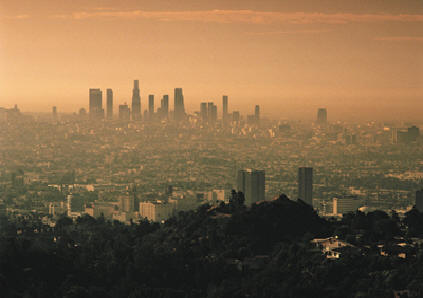
\includegraphics[scale=0.8]{smog}
\end{figure}
\end{frame}

\begin{frame}{Health Impacts}
\begin{figure}[H]
\centering
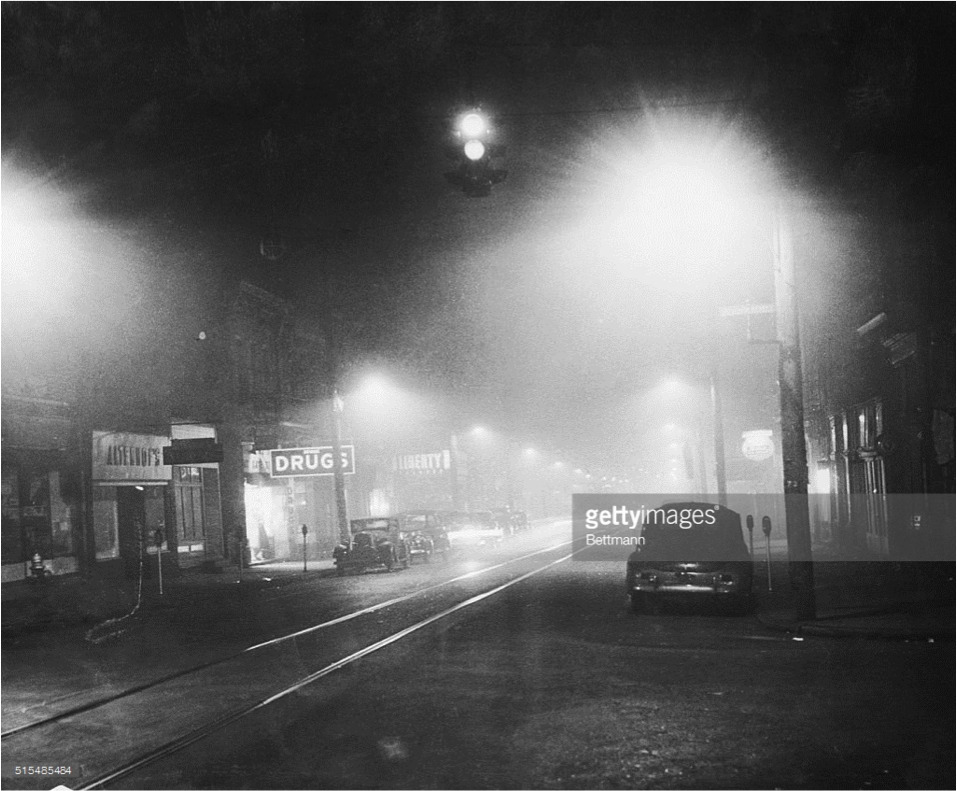
\includegraphics[scale=0.3]{19481029pm.png}
\caption{Donora, PA at noon on October 29, 1948}
\label{fig:locations}
\end{figure}

\begin{itemize}
\item 20 people died, thousands were sickened by smog from a steel mill.
\item PM$_{2.5}$ one of the most harmful pollutants, can get lodged in lungs and cause respiratory problems
\end{itemize}
\end{frame}


\begin{frame}{PM and AOD}

\begin{figure}[H]
\centering
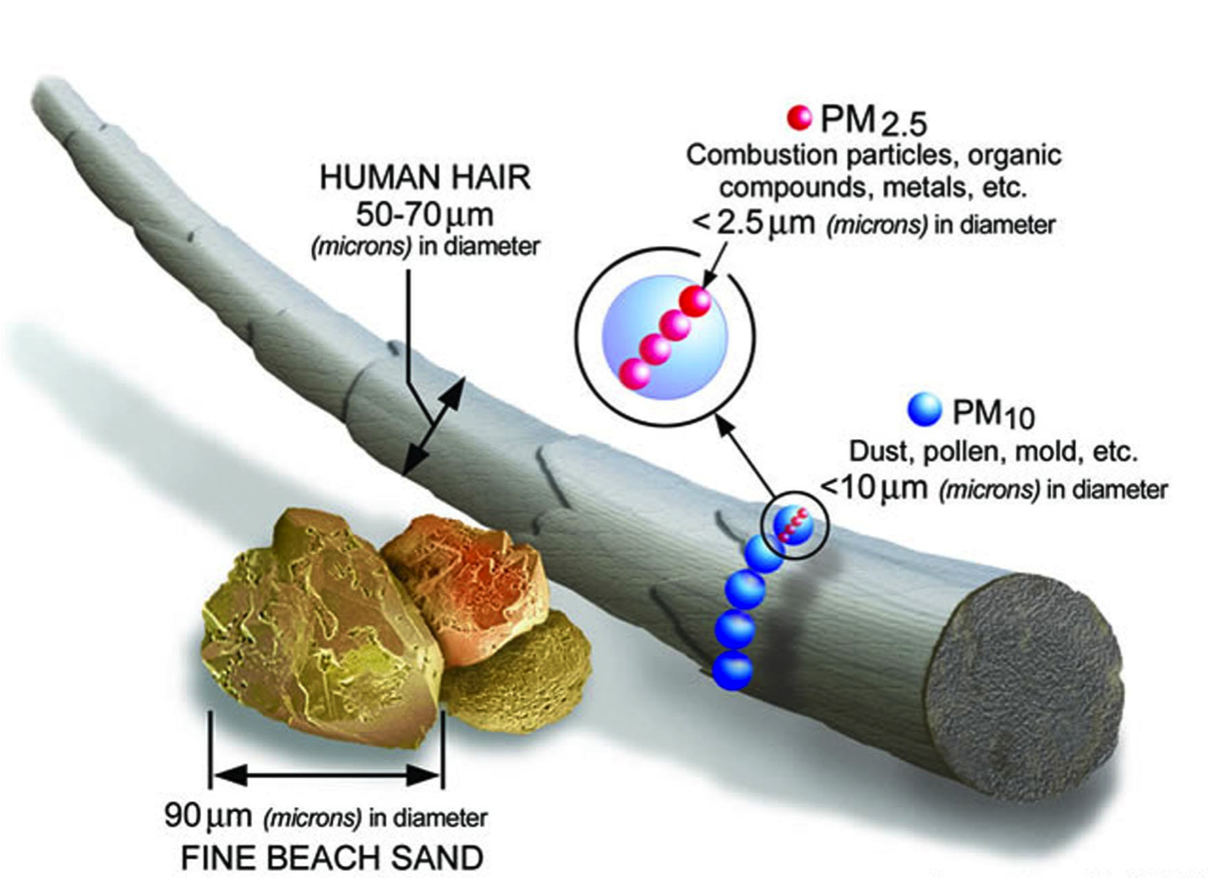
\includegraphics[scale=0.3]{hair.png}
\caption{Size of PM$_{2.5}$ compared to other particulate matter}
\label{fig:locations}
\end{figure}

\begin{itemize}
\item PM$_{2.5}$ is a particulate matter that is less than $2.5$ micrometers in diameter.
\item Aerosol Optical Depth (AOD) measures the amount of light from the sun blocked by dust and pollutants.
\end{itemize}
\end{frame}
%--------------------------------------------------------------------------------------------------------------
\begin{frame}
\begin{figure}[H]
\centering
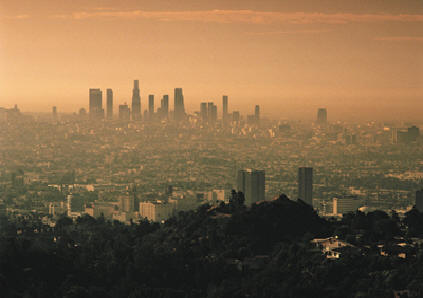
\includegraphics[scale=0.3]{smog.png}
\caption{Size of PM$_{2.5}$ compared to other particulate matter}
\label{fig:locations}
\end{figure}
\begin{itemize}
\item The Clean Air Act imposes a national standard of permissible amount of PM$_{2.5}$. 
\item Sites in California, such as in the Los Angeles area consistently violate this standard.
\item Want to investigate the possibility of external impact by international air travel of PM$_{2.5}$.
\end{itemize}
\end{frame}

%\subsection*{Background}
\begin{frame}{Background}
\begin{itemize}

\item Clean Air Act
\begin{itemize}
\item California violates it
\item China to blame?
\end{itemize}
\item Measure pollutants on land, near California coast
\item Compare with satellite measurements
\item informative picture - LA smog
\end{itemize}
\end{frame}
%--------------------------------------------------------------------------------------------------------------
\subsection*{Background}
\begin{frame}{PM and AOD}
\begin{itemize}

\item PM$_{2.5}$ is a particulate matter that is less than $2.5$ micrometers in diameter.

\begin{figure}[H]
\centering
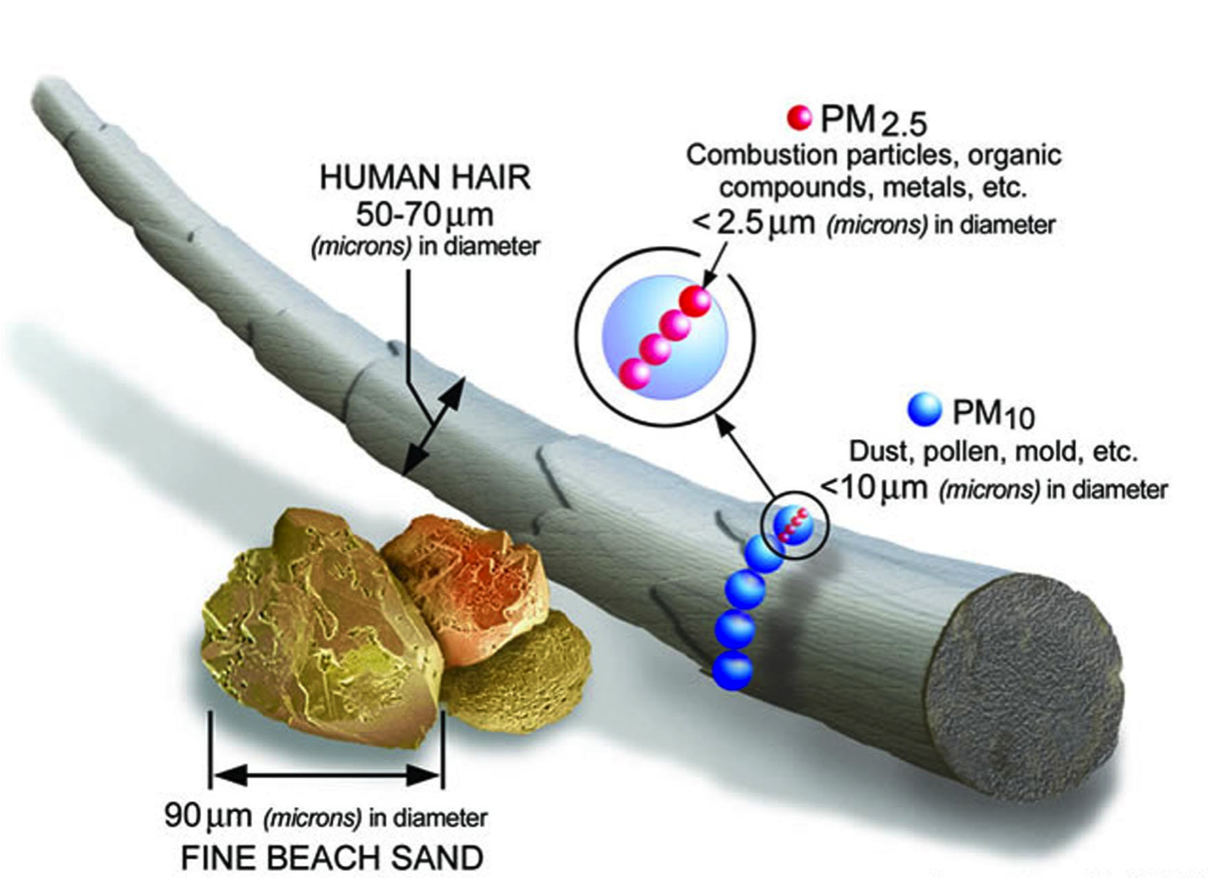
\includegraphics[scale=0.35]{hair.png}
\caption{Size of PM$_{2.5}$ compared to other particulate matter}
\label{fig:locations}
\end{figure}


\item Aerosol Optical Depth (AOD) measures the amount of light from the sun blocked by dust and pollutants.

\end{itemize}
\end{frame}



%------------------------------------------Data Sources--------------------------------------------------------

\section{Data Sources}
\begin{frame}{PM$_{2.5}$ }
\begin{figure}
\centering
\includegraphics[scale=0.3]{AllPMsites} \hspace{0.4mm}
\end{figure}

\begin{itemize}	
\item Ground sites of PM$_{2.5}$ measurements, as collected by EPA
\item Data collected either daily, every three days or every six days.
\end{itemize}	
\end{frame}


%--------------------------------------------------------------------------------------------------------------
\begin{frame}{AOD}
\begin{figure}[H]
\centering
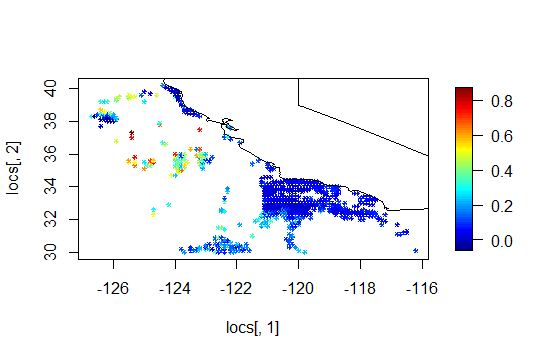
\includegraphics[scale=0.5]{AODpoints_06012009.png}
\caption{AOD readings on Jun 6, 2009}
\label{fig:locations}
\end{figure}

\begin{itemize}	
\item AOD data collected over Pacific Ocean, near coast of California.
\item Satellites travel around the Earth once every 16 days.
\item AOD data is collected at each location least twice a month.
\end{itemize}		
\end{frame}

%------------------------------------------Methods--------------------------------------------------------
\section{Methods}
\begin{frame}{Data Cleaning}
\begin{figure}[H]
\centering
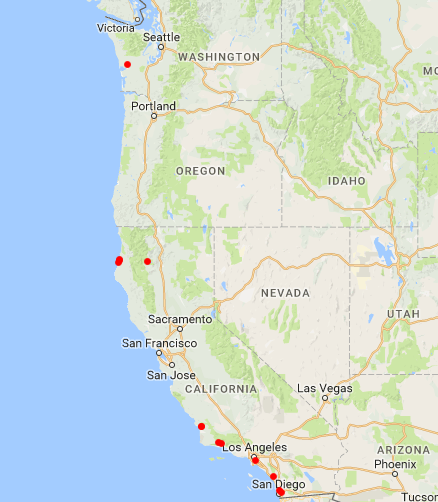
\includegraphics[scale=0.25]{figs/pm13.png} 
\hspace{1mm}
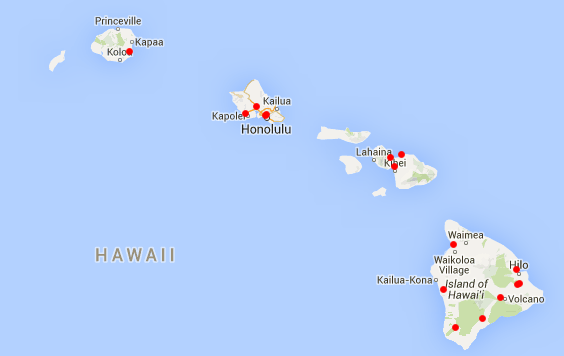
\includegraphics[scale=0.3]{figs/mappmsiteshawaii.jpg}
\caption{(left) CA PM$_{2.5}$ sites we compared with AOD data, (right) Hawaii PM$_{2.5}$ sites we compared with AOD data}
\end{figure}

\begin{itemize}

\item Picked PM sites closest to coast ($13$ in California, $9$ in Hawaii)
\item Found closest locations of AOD measurements to these sites
\item Matched data by date of AOD/PM readings

\end{itemize}
\end{frame}

%--------------------------------------------------------------------------------------------------------------
\begin{frame}{Covariates}
\begin{itemize}	
\item wind speed and direction
\item humidity
\item planetary boundary layer height
\item air temperature
\item added values of these measures at each location at each date
\end{itemize}
\end{frame}
%------------------------------------------Models-----------------------------------------------------------
\iffalse
\section{Models}
\begin{frame}{Models}
\begin{itemize}	
\item PM$_{2.5}$ time series
\item add gif here
\end{itemize}
\end{frame}
%--------------------------------------------------------------------------------------------------------------
\begin{frame}{Models}
\begin{itemize}	
\item Spatial Interpolation of PM$_{2.5}$
\item add gif/image here
\end{itemize}
\end{frame}
%--------------------------------------------------------------------------------------------------------------
\begin{frame}{Models}
\begin{itemize}	
\item Relationships between AVHRR AOD and surface PM
\item Yu - add stuff
\end{itemize}
\end{frame}
\fi
%------------------------------------------Experiments-----------------------------------------------------------
\section{Experiments}
\subsection{PM$_{2.5}$ time series}

\begin{frame}{PM$_{2.5}$ Time Series}
\begin{figure}
\centering
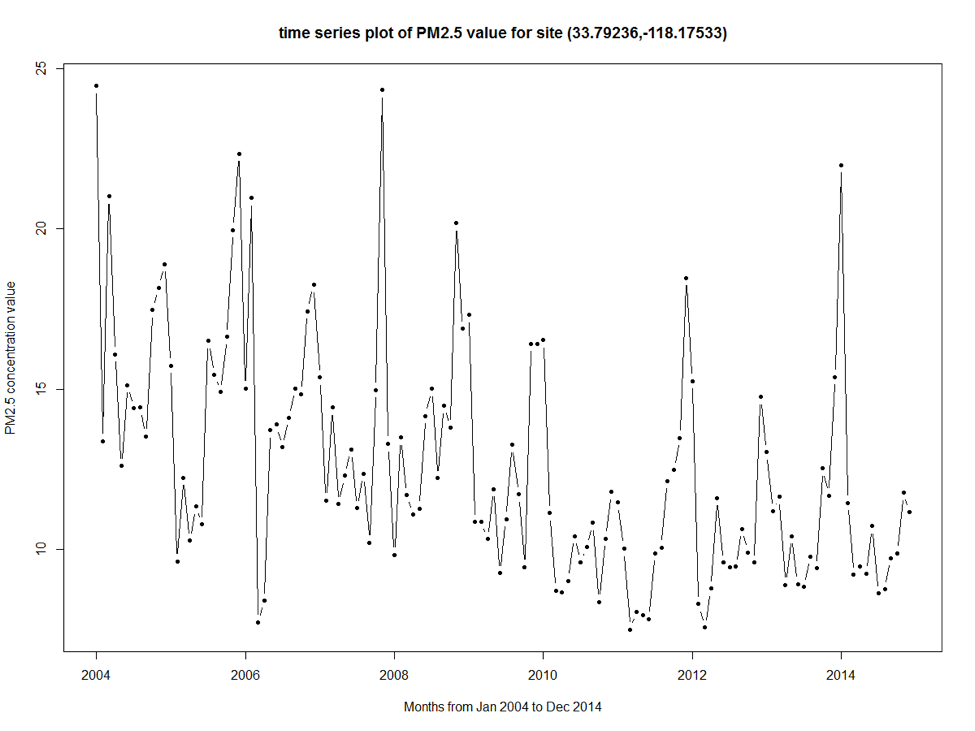
\includegraphics[width=70mm]{figs/ts1.png}
\end{figure}
\begin{itemize}
\item Goal is to make predictions about PM$_{2.5}$ in $2015$.
\item Overall pollution appears to be decreasing.
\item Seasonal variations are observed.
\item Two methods used -- Holt-Winter Exponential smoothing and ARIMA model 
\end{itemize}  
\end{frame}



\begin{frame}{Holt-Winters Exponential Smoothing}
\begin{figure}
\centering
%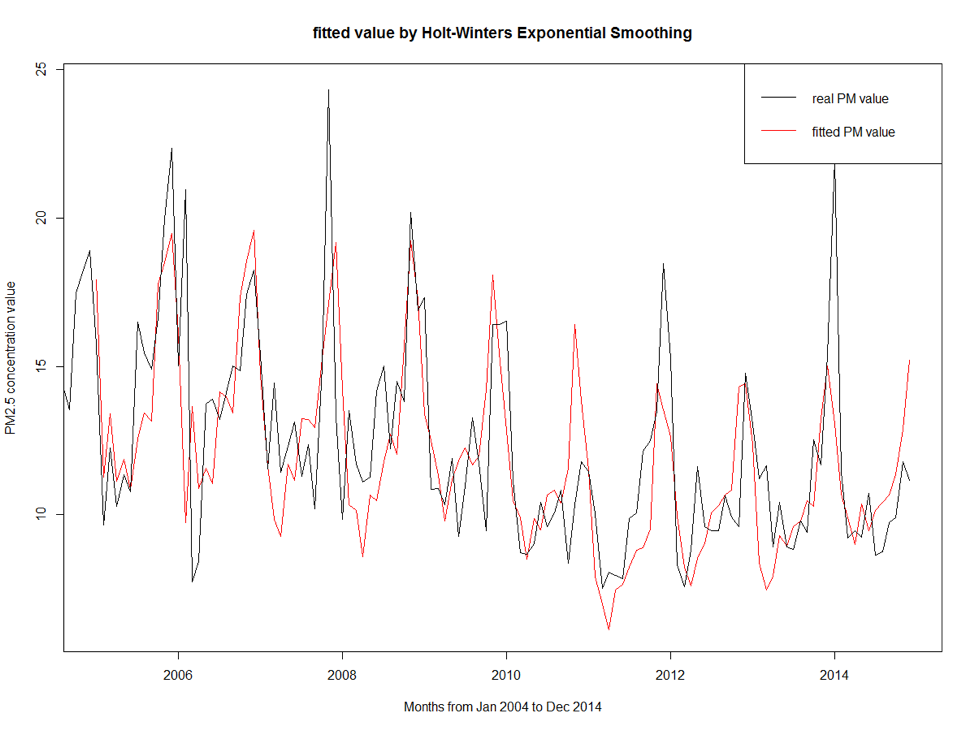
\includegraphics[width=0.9\linewidth, height=30mm]{figs/ts2.png} \vspace{2mm}
%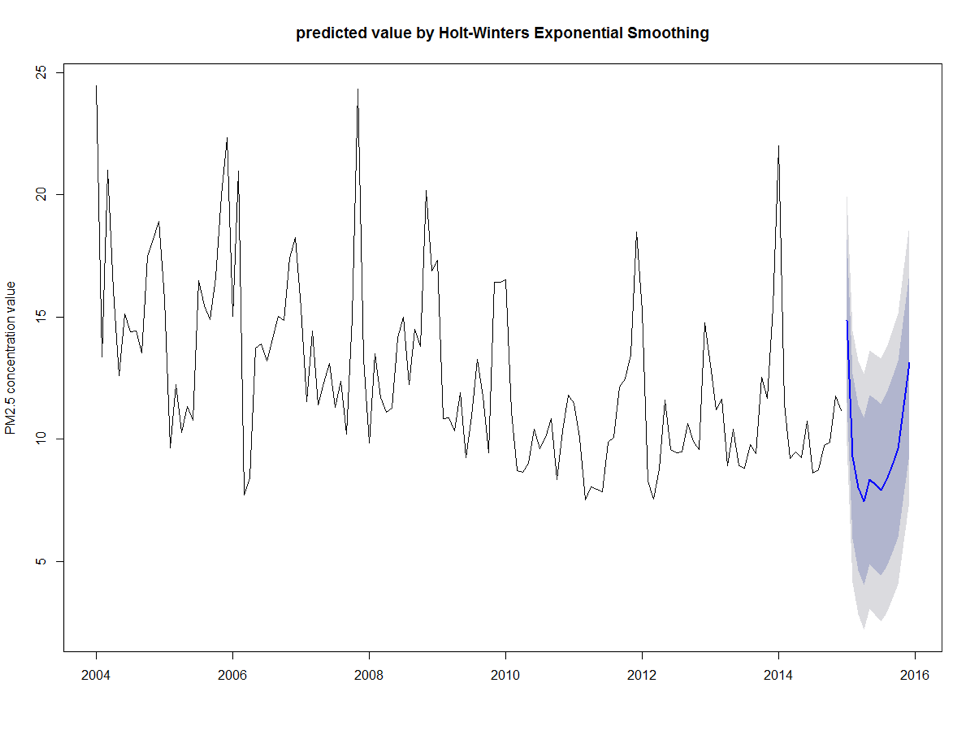
\includegraphics[width=0.9\linewidth, height=30mm]{figs/ts3.png}
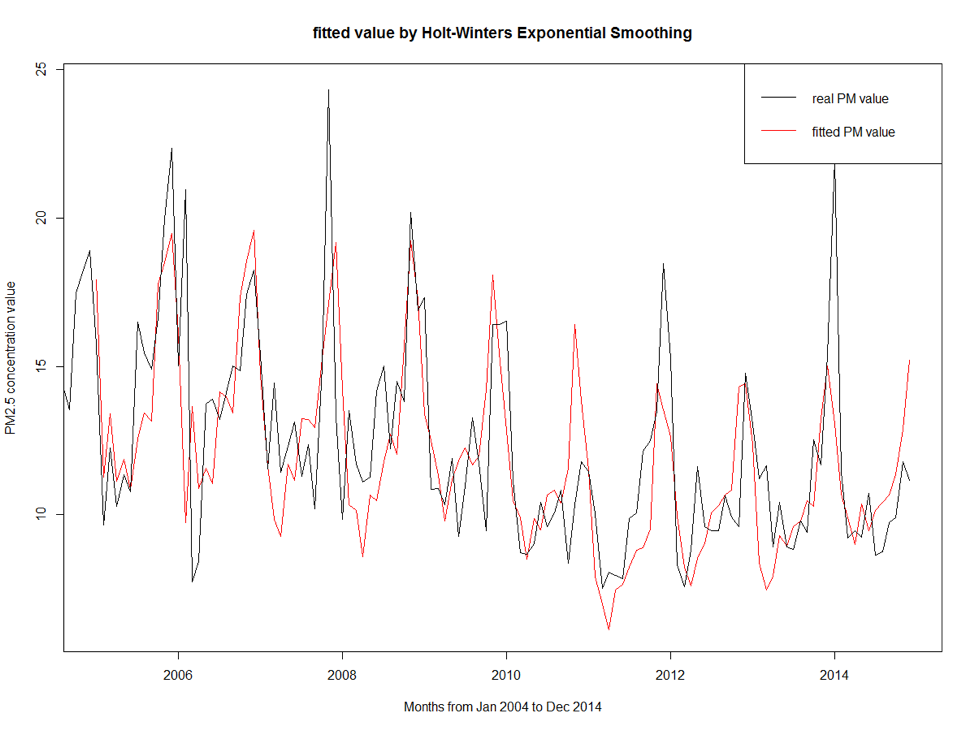
\includegraphics[scale=0.25]{figs/ts2.png} \vspace{2mm}
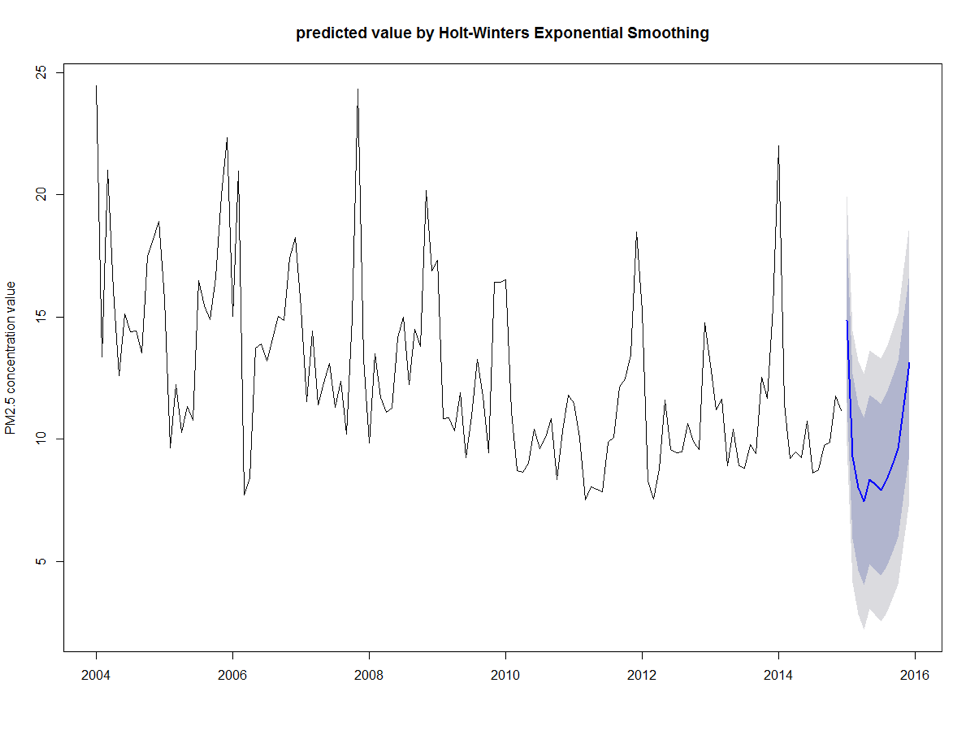
\includegraphics[scale=0.25]{figs/ts3.png}
\end{figure}
\begin{itemize}
\item Mean square error is $5.5$ but the mean of PM$_{2.5}$ values is 12.6
\item Similar result observed using different method - ARIMA.
\item PM$_{2.5}$ dataset itself not sufficient to make predictions
\item This motivates using covariates and AOD data.
\end{itemize}  
\end{frame}




\subsection{AOD and PM$_{2.5}$ relations}

\frame{\frametitle{$\PM$ vs AOD}
\begin{itemize} 
\setlength\itemsep{2.5em}
\item {\cub Goal} - relationship between ${\cub \PM}$ and {\cub AOD} in presence of other meteorological variables. 
\item Response variable - ${\cub \PM}$ - ``What we want to predict''
\item Covariates - ``What we use to predict'' 
\begin{itemize} 
\setlength\itemsep{1.5em}
\item continuous variables: {\cub wind direction, wind velocity, relative humidity, air temperature}
\item factors: {\cub season} --  a discrete variable that models  seasonality. 
\end{itemize}
\item Model the relationship at a particular ${\cub \PM}$ site or combine data from two nearby ${\cub \PM}$ sites along the west coast of United States. 
\end{itemize}
}

\frame{\frametitle{Snapshot of the dataset}
\begin{figure}[h]
\centering
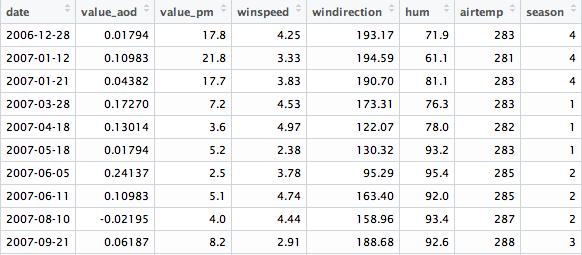
\includegraphics[width = 110mm]{figs/calidata.jpeg}
\end{figure}
\begin{itemize} 
\item ${\cub \PM}$ sites' coordinates near Eureka, CA - (40.8, -124) and (40.9, -123)
\item This site was chosen since it provides best fits. 
\end{itemize}
}

\frame{\frametitle{Preliminary Analysis I}
\begin{figure}[h]
\centering
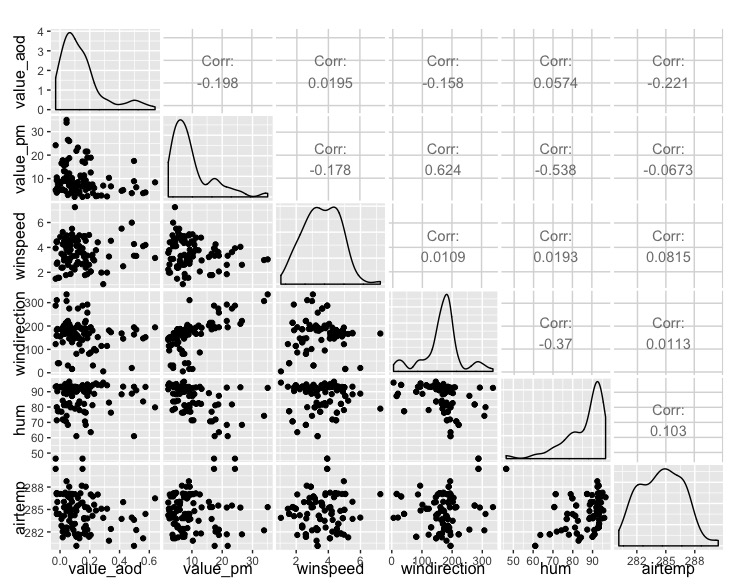
\includegraphics[scale=0.34]{figs/pairs.jpeg}
\end{figure}
\begin{itemize} 
\item Shows nonlinear relationships between covariates and responses. 
\item skewed data, outliers. 
\end{itemize}}

\frame{\frametitle{Statistical Model I}

{\cub \large Multiple Linear Regression Model}  
\begin{figure}[h]
\centering
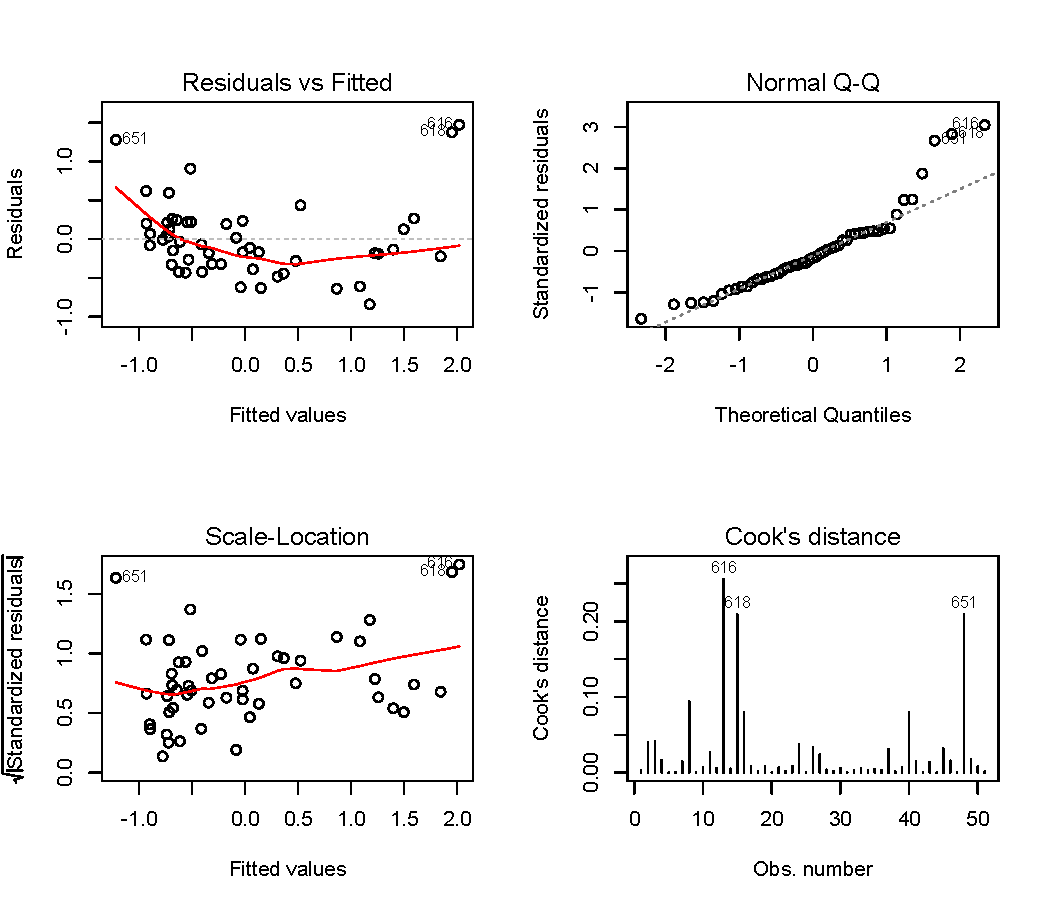
\includegraphics[scale=0.35]{figs/residual.pdf}
\caption{Some model diagnostics}
\end{figure}
{\large Multiple linear regression does not provide good fits.}
 
}

\frame{\frametitle{Statistical Model II}
{\cub \large Generalized Additive Model}  
\begin{figure}[h]
\centering
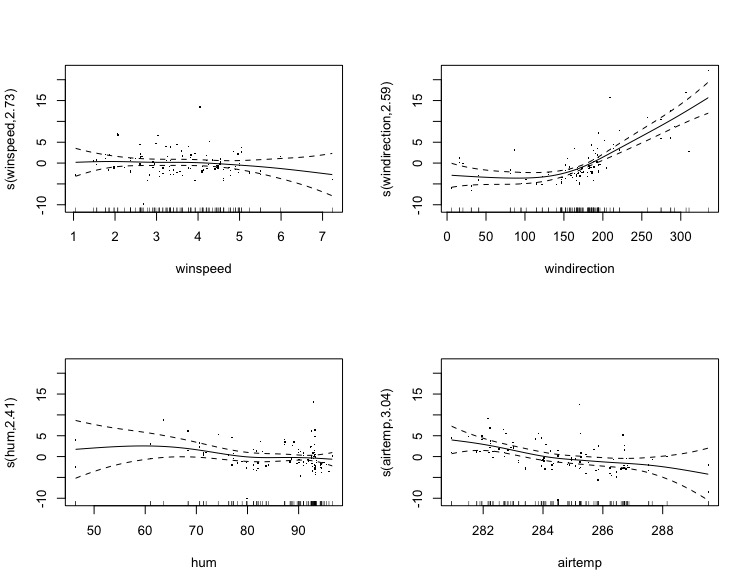
\includegraphics[width=80mm]{figs/pred.jpeg}
\end{figure}

% \begin{itemize}
%\item {\cub wind speed, wind direction, relative humidity} use something something less regular than a quadratic term and each of them require about two and half degrees of freedom.  
%\end{itemize}
}





%-------------------------------------------Conclusions---------------------------------------------------------
\section{Conclusions}
\begin{frame}{Conclusions and future work}

\textbf{Conclusions}

\begin{itemize}

\item AOD has a linear relationship with the PM$_{2.5}$ measurements.
\item Meteorological information is also important in predicting PM$_{2.5}$ (particularly wind speed).
\item GAM model better than multivariate linear regression model better than mixed effects model.
\end{itemize}

\vspace{5mm}
\textbf{Future work}
\begin{itemize}

\item Perform analysis on Hawaii sites. 
\item Use data from more years to train our model.
\item Performing spatio-temporal analysis. 
\end{itemize}

\end{frame}



%--------------------------------------------------------------------------------------------------------------
\begin{frame}{Acknowledgments}
\begin{itemize}
\item Faculty mentors
\item EPA -- Elizabeth Mannshardt and 
\item We would like to thank the NOAA, specifically Jessica Matthews for helping to explain the satellite data
\item IMSM
\item NSF
\end{itemize}
\end{frame}

%--------------------------------------------------------------------------------------------------------------
\begin{frame}{References}
	\begin{thebibliography}{99}
	\beamertemplatearticlebibitems
	
	\bibitem{liu} 
	
	\bibitem{noaa} National Centers for Environmental Information. National Oceanic and Atmospheric Administration. Department of Commerce, n.d. Web. 23 July 2016. \textit{https://www.ncdc.noaa.gov/cdr/atmospheric/avhrr-aerosol-optical-thickness}.
	
\bibitem{epa} United States Environmental Protection Agency. AirData. EPA, 5 July 2016. Web. 23 July 2016. \textit{https://www3.epa.gov/airdata/}.
	

	\end{thebibliography}
%use this as reference for citations	
%	
%	\bibitem{selfridge} \textcolor{black}{J. Brillhart; D. H. Lehmer; J. L. Selfridge; B. Tuckerman; S. S. Wagstaff, Jr., 
%	Factorizations of $b^n \pm 1$, $b = 2,3,5,6,7,10,11,12$ Up to High Powers, $3\rdd$ edition, Contemporary 
%	Mathematics, Vol. 22, American Math. Soc., Providence, 2002.}
%	
%	\beamertemplatearticlebibitems
%	\bibitem{erdos} \textcolor{black}{P. Erd\H{o}s, On integers of the form $2^k + p$ and some related problems, 
%	\textit{Summa Brasil. Math.} \textbf{2} (1950) 113--123.}
%	
%	\bibitem{mkozekRS} \textcolor{black}{M. Filaseta, C. Finch, M. Kozek, On powers associated with Sierpi\'nski numbers, 
%	Riesel numbers and Polignac's conjecture. \textit{J. Number Theory} \textbf{128} (2008), no. 7, 1916--1940.}
%	
%	\bibitem{marksenior} \textcolor{black}{M. Filaseta; M. Kozek; C. Nicol; J. Selfridge, Composites that remain composite 
%	after changing a digit, \textit{J. Comb. Number Theory} \textbf{2} (2010), no. 1, 25--36 (2011).}
%	\end{thebibliography}
\end{frame}

\end{document}
